\documentclass[11pt]{article}

\usepackage[T1]{fontenc}
\usepackage[utf8]{inputenc}
\usepackage{lmodern}
\usepackage{microtype}
\usepackage[margin=0.82in]{geometry}
\usepackage{amsmath,amssymb,mathtools}
\usepackage{booktabs}
\usepackage{array}
\usepackage{enumitem}
\usepackage[most]{tcolorbox}
\usepackage{tikz}
\usetikzlibrary{arrows.meta,calc,decorations.pathreplacing,positioning}
\usepackage{fancyhdr}
\usepackage{hyperref}
\usepackage{needspace}
\usepackage{graphicx}
\usepackage{multicol}

\hypersetup{
  colorlinks=true,
  linkcolor=blue!55!black,
  urlcolor=blue!55!black,
  pdftitle={Exercise 9.9: Self-Generalizations of Holder's Inequality},
  pdfauthor={OpenAI}
}

\setlength{\parindent}{0pt}
\setlength{\parskip}{0.62em}
\setlist[itemize]{leftmargin=1.55em,itemsep=0.25em,topsep=0.25em}
\setlist[enumerate]{leftmargin=1.8em,itemsep=0.35em,topsep=0.3em}
\allowdisplaybreaks
\setcounter{tocdepth}{1}

\pagestyle{fancy}
\fancyhf{}
\lhead{Exercise 9.9 Tutorial}
\rhead{H\"older's Inequality}
\cfoot{\thepage}
\setlength{\headheight}{14pt}

\definecolor{navy}{RGB}{24,55,93}
\definecolor{softblue}{RGB}{235,244,252}
\definecolor{softgreen}{RGB}{236,248,239}
\definecolor{softyellow}{RGB}{255,249,226}
\definecolor{softred}{RGB}{253,239,239}
\definecolor{softgray}{RGB}{245,246,248}
\definecolor{softpurple}{RGB}{245,239,251}

\newtcolorbox{problemBox}{
  enhanced,
  colback=softblue,
  colframe=navy,
  boxrule=0.8pt,
  arc=2mm,
  title=The problem,
  fonttitle=\bfseries,
  breakable
}

\newtcolorbox{ideaBox}[1][Key idea]{
  enhanced,
  colback=softgreen,
  colframe=green!45!black,
  boxrule=0.7pt,
  arc=2mm,
  title={#1},
  fonttitle=\bfseries,
  breakable
}

\newtcolorbox{warningBox}[1][Watch out]{
  enhanced,
  colback=softyellow,
  colframe=orange!65!black,
  boxrule=0.7pt,
  arc=2mm,
  title={#1},
  fonttitle=\bfseries,
  breakable
}

\newtcolorbox{solutionBox}[1][Solution step]{
  enhanced,
  colback=white,
  colframe=navy!75,
  boxrule=0.8pt,
  arc=2mm,
  title={#1},
  fonttitle=\bfseries,
  breakable
}

\newtcolorbox{definitionBox}[1][Definition]{
  enhanced,
  colback=softgray,
  colframe=black!45,
  boxrule=0.6pt,
  arc=2mm,
  title={#1},
  fonttitle=\bfseries,
  breakable
}

\newtcolorbox{extraBox}[1][Extra insight]{
  enhanced,
  colback=softpurple,
  colframe=purple!55!black,
  boxrule=0.7pt,
  arc=2mm,
  title={#1},
  fonttitle=\bfseries,
  breakable
}

\newcommand{\abs}[1]{\left|#1\right|}
\newcommand{\norm}[1]{\left\lVert #1\right\rVert}
\newcommand{\R}{\mathbb{R}}
\newcommand{\pointprod}{\mathbin{\odot}}

\begin{document}

\begin{center}
  {\LARGE\bfseries Exercise 9.9: Self-Generalizations of H\"older's Inequality}\\[0.35em]
  {\Large Why reciprocal exponents add when sequences are multiplied}\\[0.7em]
  {\large A step-by-step tutorial for a high-school reader}
\end{center}

\vspace{0.4em}

\begin{ideaBox}[What you will learn]
By the end of this tutorial, you will be able to:
\begin{itemize}
  \item read expressions such as \(\left(\sum a_j^p\right)^{1/p}\);
  \item recognize a pair of \emph{conjugate exponents};
  \item turn the relation \(1/p+1/q=1/r\) into the usual H\"older relation;
  \item prove the two-factor inequality in part (a) line by line;
  \item prove the three-factor inequality in part (b) by grouping two factors;
  \item understand the general rule that reciprocal exponents behave like a budget.
\end{itemize}
\end{ideaBox}

\tableofcontents
\newpage

\section{The exercise, stated carefully}

\begin{problemBox}
Let \(a_1,\ldots,a_n\), \(b_1,\ldots,b_n\), and \(c_1,\ldots,c_n\) be nonnegative real numbers.

\textbf{(a)} Suppose \(p,q,r>0\), with \(p>r\), \(q>r\), and
\[
  \frac1p+\frac1q=\frac1r.
\]
Prove that
\[
 \boxed{\displaystyle
 \left(\sum_{j=1}^{n}(a_jb_j)^r\right)^{1/r}
 \leq
 \left(\sum_{j=1}^{n}a_j^p\right)^{1/p}
 \left(\sum_{j=1}^{n}b_j^q\right)^{1/q}.}
 \tag{A}
\]

\textbf{(b)} Suppose \(p,q,r>1\) and
\[
  \frac1p+\frac1q+\frac1r=1.
\]
Prove that
\[
 \boxed{\displaystyle
 \sum_{j=1}^{n}a_jb_jc_j
 \leq
 \left(\sum_{j=1}^{n}a_j^p\right)^{1/p}
 \left(\sum_{j=1}^{n}b_j^q\right)^{1/q}
 \left(\sum_{j=1}^{n}c_j^r\right)^{1/r}.}
 \tag{B}
\]
\end{problemBox}

\begin{warningBox}[What if the numbers can be negative?]
If the entries are arbitrary real numbers, noninteger powers such as \(a_j^p\) may not even be real when \(a_j<0\). The standard real-valued versions use absolute values:
\[
 \left(\sum_{j=1}^{n}\abs{a_jb_j}^{r}\right)^{1/r}
 \leq
 \left(\sum_{j=1}^{n}\abs{a_j}^{p}\right)^{1/p}
 \left(\sum_{j=1}^{n}\abs{b_j}^{q}\right)^{1/q},
 \tag{A$'$}
\]
and
\[
 \abs{\sum_{j=1}^{n}a_jb_jc_j}
 \leq
 \left(\sum_{j=1}^{n}\abs{a_j}^{p}\right)^{1/p}
 \left(\sum_{j=1}^{n}\abs{b_j}^{q}\right)^{1/q}
 \left(\sum_{j=1}^{n}\abs{c_j}^{r}\right)^{1/r}.
 \tag{B$'$}
\]
We prove the nonnegative form printed in the exercise. Applying that proof to \(\abs{a_j}\), \(\abs{b_j}\), and \(\abs{c_j}\), together with the triangle inequality, gives the stronger real-valued forms above.
\end{warningBox}

\section{The small amount of background we need}

\subsection{Finite sequences and pointwise products}

A finite sequence is simply an ordered list. For example,
\[
  a=(a_1,a_2,a_3)=(1,2,4),
  \qquad
  b=(b_1,b_2,b_3)=(3,5,2).
\]
Their \emph{pointwise product} is obtained by multiplying entries with the same index:
\[
  ab=(a_1b_1,a_2b_2,a_3b_3)=(3,10,8).
\]
The symbol \(j\) in a sum tells us which matching pair is being used:
\[
  \sum_{j=1}^{3}a_jb_j=a_1b_1+a_2b_2+a_3b_3.
\]

\subsection{Power-sum sizes}

For a nonnegative sequence \(a=(a_1,\ldots,a_n)\) and a positive number \(p\), define
\[
  \norm{a}_p:=\left(\sum_{j=1}^{n}a_j^p\right)^{1/p}.
  \tag{1}
\]
For example, if \(a=(1,2)\), then
\[
 \norm{a}_1=1+2=3,
 \qquad
 \norm{a}_2=\sqrt{1^2+2^2}=\sqrt5,
 \qquad
 \norm{a}_4=(1^4+2^4)^{1/4}=17^{1/4}.
\]
When \(p\geq1\), this is called the \(\ell^p\)-norm of the sequence. Part (a) allows \(0<r<1\), in which case the same formula is still useful, although mathematicians do not technically call it a norm.

With this notation, part (a) is the compact statement
\[
  \norm{ab}_r\leq \norm{a}_p\norm{b}_q.
  \tag{2}
\]

\subsection{Two exponent rules used repeatedly}

For \(x\geq0\) and positive exponents, we use
\[
  (x^\alpha)^\beta=x^{\alpha\beta}.
  \tag{3}
\]
Two instances will be especially important:
\[
  \left(a_j^r\right)^{p/r}=a_j^{r(p/r)}=a_j^p,
  \tag{4}
\]
and, for \(X\geq0\),
\[
  \left(X^{r/p}\right)^{1/r}=X^{(r/p)(1/r)}=X^{1/p}.
  \tag{5}
\]
The fractions \(p/r\) and \(r/p\) look similar, so it is worth slowing down whenever they appear.

\subsection{Conjugate exponents}

\begin{definitionBox}[Conjugate exponents]
Numbers \(P,Q>1\) are called \emph{conjugate exponents} when
\[
  \frac1P+\frac1Q=1.
  \tag{6}
\]
\end{definitionBox}

Some common pairs are
\[
\begin{array}{c|c|c}
P & Q & 1/P+1/Q\\ \hline
2 & 2 & 1/2+1/2=1\\[2pt]
3 & 3/2 & 1/3+2/3=1\\[2pt]
4 & 4/3 & 1/4+3/4=1
\end{array}
\]
If one exponent is \(P>1\), its conjugate is
\[
  Q=\frac{P}{P-1}.
\]

\subsection{The ordinary two-factor H\"older inequality}

The theorem that this exercise asks us to reuse is the following.

\begin{definitionBox}[Ordinary H\"older inequality]
Let \(P,Q>1\) satisfy \(1/P+1/Q=1\). For nonnegative numbers \(x_j,y_j\),
\[
  \boxed{\displaystyle
  \sum_{j=1}^{n}x_jy_j
  \leq
  \left(\sum_{j=1}^{n}x_j^P\right)^{1/P}
  \left(\sum_{j=1}^{n}y_j^Q\right)^{1/Q}.}
  \tag{H}
\]
\end{definitionBox}

When \(P=Q=2\), this is the familiar Cauchy--Schwarz inequality:
\[
  \sum_{j=1}^{n}x_jy_j
  \leq
  \sqrt{\sum_{j=1}^{n}x_j^2}\,
  \sqrt{\sum_{j=1}^{n}y_j^2}.
\]
The exercise does not ask us to reprove (H). Our task is to choose new sequences and new exponents so that (H) produces the desired formulas.

\begin{ideaBox}[The strategy in one sentence]
Do not force the original exponents \(p,q,r\) directly into H\"older's inequality. First \emph{rescale the exponents} until their reciprocals add to \(1\).
\end{ideaBox}

\section{The exponent-budget picture}

Relations among reciprocal exponents are easier to remember if we imagine a bar whose total length is being divided into pieces.

\subsection{Part (a): scale a total of \(1/r\) into a total of \(1\)}

The hypothesis says
\[
  \frac1p+\frac1q=\frac1r.
\]
Multiplying every term by \(r\) gives
\[
  \frac{r}{p}+\frac{r}{q}=1.
  \tag{7}
\]
This is exactly the conjugate-exponent pattern required by ordinary H\"older.

\begin{center}
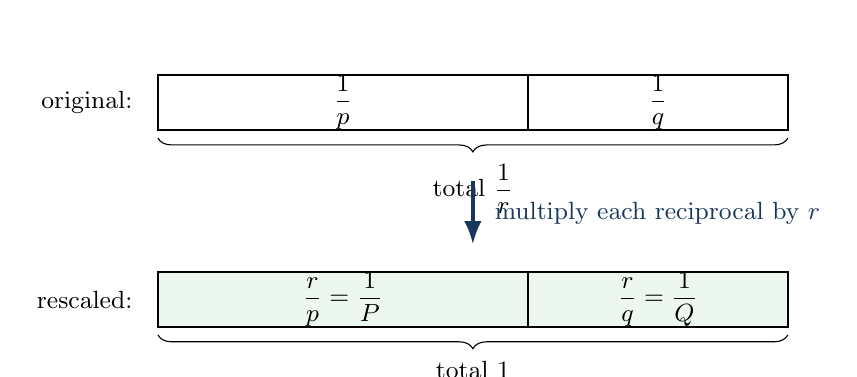
\begin{tikzpicture}[x=1cm,y=1cm,>=Latex,font=\small]
  \node[anchor=east] at (-0.2,1.35) {original:};
  \draw[thick] (0,1) rectangle (8,1.7);
  \draw[thick] (4.7,1)--(4.7,1.7);
  \node at (2.35,1.35) {$\dfrac1p$};
  \node at (6.35,1.35) {$\dfrac1q$};
  \draw[decorate,decoration={brace,amplitude=5pt,mirror}] (0,0.9)--(8,0.9)
    node[midway,below=6pt] {total $\dfrac1r$};

  \draw[->,very thick,navy] (4,0.35)--(4,-0.45)
    node[midway,right=4pt] {multiply each reciprocal by $r$};

  \node[anchor=east] at (-0.2,-1.15) {rescaled:};
  \draw[thick,fill=softgreen] (0,-1.5) rectangle (8,-0.8);
  \draw[thick] (4.7,-1.5)--(4.7,-0.8);
  \node at (2.35,-1.15) {$\dfrac{r}{p}=\dfrac1P$};
  \node at (6.35,-1.15) {$\dfrac{r}{q}=\dfrac1Q$};
  \draw[decorate,decoration={brace,amplitude=5pt,mirror}] (0,-1.6)--(8,-1.6)
    node[midway,below=6pt] {total $1$};
\end{tikzpicture}
\end{center}

The correct new exponents are therefore
\[
  P=\frac{p}{r},
  \qquad
  Q=\frac{q}{r},
  \tag{8}
\]
because then \(1/P=r/p\) and \(1/Q=r/q\).

\subsection{Part (b): combine two pieces first}

The hypothesis in part (b) divides a total reciprocal budget of \(1\) into three pieces:
\[
  \frac1p+\frac1q+\frac1r=1.
\]
We will combine the first two pieces and call their total \(1/s\):
\[
  \frac1s:=\frac1p+\frac1q.
  \tag{9}
\]
Then
\[
  \frac1s+\frac1r=1,
  \tag{10}
\]
so \(s\) and \(r\) are conjugate exponents.

\begin{center}
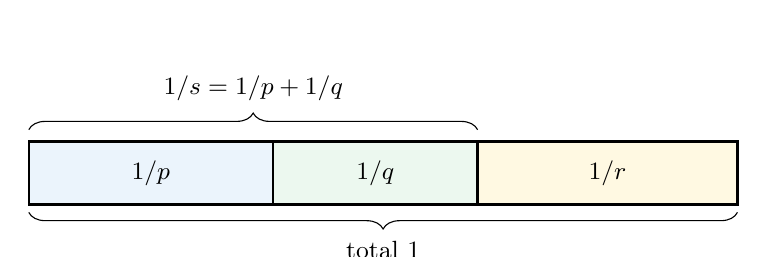
\begin{tikzpicture}[x=1cm,y=1cm,font=\small]
  \draw[thick] (0,0) rectangle (9,0.8);
  \draw[thick] (3.1,0)--(3.1,0.8);
  \draw[thick] (5.7,0)--(5.7,0.8);
  \fill[softblue] (0,0) rectangle (3.1,0.8);
  \fill[softgreen] (3.1,0) rectangle (5.7,0.8);
  \fill[softyellow] (5.7,0) rectangle (9,0.8);
  \draw[thick] (0,0) rectangle (9,0.8);
  \draw[thick] (3.1,0)--(3.1,0.8);
  \draw[thick] (5.7,0)--(5.7,0.8);
  \node at (1.55,0.4) {$1/p$};
  \node at (4.4,0.4) {$1/q$};
  \node at (7.35,0.4) {$1/r$};
  \draw[decorate,decoration={brace,amplitude=6pt}] (0,0.95)--(5.7,0.95)
    node[midway,above=7pt] {$1/s=1/p+1/q$};
  \draw[decorate,decoration={brace,amplitude=6pt,mirror}] (0,-0.1)--(9,-0.1)
    node[midway,below=7pt] {total $1$};
\end{tikzpicture}
\end{center}

This picture tells us the proof plan: first control the product \(a_jb_j\) in the \(s\)-power sum, and then combine that product with \(c_j\).

\section{Part (a): the two-factor generalization}

We assume throughout this section that
\[
  p,q,r>0,
  \qquad p>r,
  \qquad q>r,
  \qquad
  \frac1p+\frac1q=\frac1r.
  \tag{11}
\]

\begin{solutionBox}[Step 1: manufacture conjugate exponents]
Define
\[
  P:=\frac{p}{r},
  \qquad
  Q:=\frac{q}{r}.
  \tag{12}
\]
Because \(p>r\) and \(q>r\), we have \(P>1\) and \(Q>1\). Also,
\[
 \frac1P+\frac1Q
 =\frac{r}{p}+\frac{r}{q}
 =r\left(\frac1p+\frac1q\right)
 =r\cdot\frac1r
 =1.
 \tag{13}
\]
Thus \(P,Q\) are conjugate exponents, exactly as ordinary H\"older requires.
\end{solutionBox}

\begin{solutionBox}[Step 2: choose the sequences to which H\"older will be applied]
Set
\[
  x_j:=a_j^r,
  \qquad
  y_j:=b_j^r.
  \tag{14}
\]
Then
\[
  x_jy_j=a_j^rb_j^r=(a_jb_j)^r.
  \tag{15}
\]
This makes the left side of ordinary H\"older equal to the sum appearing inside the left side of (A).
\end{solutionBox}

\begin{solutionBox}[Step 3: apply ordinary H\"older]
Applying (H) to the sequences \((x_j)\) and \((y_j)\) with exponents \(P,Q\) gives
\[
\begin{aligned}
 \sum_{j=1}^{n}(a_jb_j)^r
 &=\sum_{j=1}^{n}x_jy_j\\
 &\leq
 \left(\sum_{j=1}^{n}x_j^P\right)^{1/P}
 \left(\sum_{j=1}^{n}y_j^Q\right)^{1/Q}.
\end{aligned}
\tag{16}
\]
Now simplify each power:
\[
 x_j^P=(a_j^r)^{p/r}=a_j^p,
 \qquad
 y_j^Q=(b_j^r)^{q/r}=b_j^q.
 \tag{17}
\]
Also \(1/P=r/p\) and \(1/Q=r/q\). Therefore (16) becomes
\[
 \sum_{j=1}^{n}(a_jb_j)^r
 \leq
 \left(\sum_{j=1}^{n}a_j^p\right)^{r/p}
 \left(\sum_{j=1}^{n}b_j^q\right)^{r/q}.
 \tag{18}
\]
\end{solutionBox}

\begin{solutionBox}[Step 4: take the positive \(r\)-th root]
Every quantity in (18) is nonnegative. Since \(r>0\), the function \(t\mapsto t^{1/r}\) is increasing for \(t\geq0\). Taking the \(r\)-th root preserves the inequality:
\[
\begin{aligned}
 \left(\sum_{j=1}^{n}(a_jb_j)^r\right)^{1/r}
 &\leq
 \left[
 \left(\sum_{j=1}^{n}a_j^p\right)^{r/p}
 \left(\sum_{j=1}^{n}b_j^q\right)^{r/q}
 \right]^{1/r}\\[2pt]
 &=
 \left(\sum_{j=1}^{n}a_j^p\right)^{1/p}
 \left(\sum_{j=1}^{n}b_j^q\right)^{1/q}.
\end{aligned}
\tag{19}
\]
This is exactly the desired inequality (A).
\end{solutionBox}

\begin{ideaBox}[The whole proof compressed into one display]
\[
\begin{aligned}
 \sum_{j=1}^{n}(a_jb_j)^r
 &=\sum_{j=1}^{n}(a_j^r)(b_j^r)\\
 &\leq
 \left(\sum_{j=1}^{n}(a_j^r)^{p/r}\right)^{r/p}
 \left(\sum_{j=1}^{n}(b_j^r)^{q/r}\right)^{r/q}\\
 &=
 \left(\sum_{j=1}^{n}a_j^p\right)^{r/p}
 \left(\sum_{j=1}^{n}b_j^q\right)^{r/q}.
\end{aligned}
\]
The first line prepares the product; the second line is ordinary H\"older; the third line simplifies exponents. Taking the \(r\)-th root finishes the argument.
\end{ideaBox}

\subsection{Why the condition \(p,q>r\) appears}

Ordinary H\"older needs exponents greater than \(1\). Our new exponents are \(P=p/r\) and \(Q=q/r\), so we need
\[
  \frac{p}{r}>1,
  \qquad
  \frac{q}{r}>1,
\]
which is precisely \(p>r\) and \(q>r\).

In fact, once all three numbers are positive, the reciprocal equation already forces these inequalities. For example,
\[
  \frac1r=\frac1p+\frac1q>\frac1p.
\]
For positive numbers, a larger reciprocal corresponds to a smaller number, so \(r<p\). Similarly, \(r<q\).

\subsection{A concrete equality example}

Take
\[
  p=q=4,
  \qquad
  r=2.
\]
Indeed,
\[
  \frac14+\frac14=\frac12=\frac1r.
\]
Let \(a=b=(1,2)\). The left side is
\[
 \left((1\cdot1)^2+(2\cdot2)^2\right)^{1/2}
 =\sqrt{1+16}
 =\sqrt{17}.
\]
The right side is
\[
 (1^4+2^4)^{1/4}(1^4+2^4)^{1/4}
 =17^{1/4}17^{1/4}
 =\sqrt{17}.
\]
Thus equality can occur.

\subsection{When does equality occur?}

For nonzero nonnegative sequences, equality in ordinary H\"older occurs when the powered sequences are proportional. Here that condition becomes
\[
  (a_j^r)^P=\lambda(b_j^r)^Q
  \qquad\text{for every }j,
\]
or equivalently
\[
  \boxed{a_j^p=\lambda b_j^q\quad\text{for every }j}
  \tag{20}
\]
for some constant \(\lambda>0\). The example \(p=q=4\), \(a=b\) satisfies this with \(\lambda=1\).

\section{Part (b): the triple-product inequality}

Now assume
\[
  p,q,r>1,
  \qquad
  \frac1p+\frac1q+\frac1r=1.
  \tag{21}
\]
The goal is to control a product of \emph{three} sequences using the two-factor H\"older inequality.

\begin{ideaBox}[Group two factors into one]
Write
\[
  a_jb_jc_j=(a_jb_j)c_j.
\]
We will first treat \(a_jb_j\) as one sequence and pair it with \(c_j\). Part (a) will then separate \(a_j\) and \(b_j\) again.
\end{ideaBox}

\begin{solutionBox}[Step 1: define the intermediate exponent \(s\)]
Let \(s\) be defined by
\[
  \frac1s:=\frac1p+\frac1q.
  \tag{22}
\]
Using (21),
\[
  \frac1s=1-\frac1r,
\]
so
\[
  \frac1s+\frac1r=1.
  \tag{23}
\]
Thus \(s\) and \(r\) are conjugate exponents. Solving explicitly gives
\[
  s=\frac{r}{r-1}>1,
\]
because \(r>1\).
\end{solutionBox}

\begin{solutionBox}[Step 2: verify that part (a) applies to \(a\) and \(b\)]
Equation (22) has the same form as the hypothesis in part (a), with the smaller output exponent now called \(s\):
\[
  \frac1p+\frac1q=\frac1s.
\]
We also need \(p>s\) and \(q>s\). Since
\[
  \frac1s=\frac1p+\frac1q>\frac1p,
\]
and all numbers are positive, we have \(s<p\). Similarly, \(s<q\). Therefore part (a) gives
\[
  \left(\sum_{j=1}^{n}(a_jb_j)^s\right)^{1/s}
  \leq
  \left(\sum_{j=1}^{n}a_j^p\right)^{1/p}
  \left(\sum_{j=1}^{n}b_j^q\right)^{1/q}.
  \tag{24}
\]
\end{solutionBox}

\begin{solutionBox}[Step 3: pair the product \(a_jb_j\) with \(c_j\)]
Because \(1/s+1/r=1\), ordinary H\"older applied to the two sequences
\[
  x_j=a_jb_j,
  \qquad
  y_j=c_j
\]
gives
\[
\begin{aligned}
 \sum_{j=1}^{n}a_jb_jc_j
 &=\sum_{j=1}^{n}(a_jb_j)c_j\\
 &\leq
 \left(\sum_{j=1}^{n}(a_jb_j)^s\right)^{1/s}
 \left(\sum_{j=1}^{n}c_j^r\right)^{1/r}.
\end{aligned}
\tag{25}
\]
Now substitute the estimate (24) into (25):
\[
\begin{aligned}
 \sum_{j=1}^{n}a_jb_jc_j
 &\leq
 \left(\sum_{j=1}^{n}a_j^p\right)^{1/p}
 \left(\sum_{j=1}^{n}b_j^q\right)^{1/q}
 \left(\sum_{j=1}^{n}c_j^r\right)^{1/r}.
\end{aligned}
\]
This is exactly (B).
\end{solutionBox}

\begin{center}
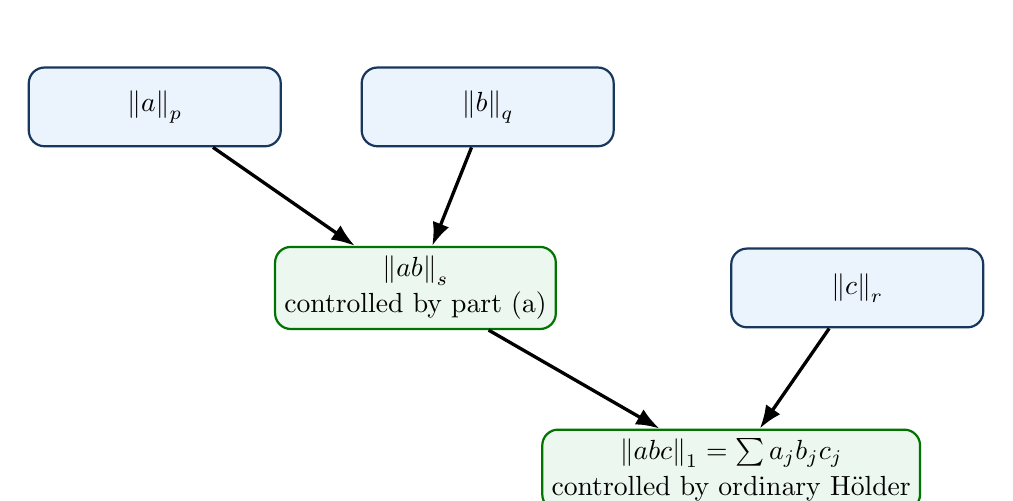
\begin{tikzpicture}[
  >=Latex,
  node distance=1.2cm and 1.0cm,
  box/.style={draw=navy,rounded corners=2mm,thick,align=center,minimum height=1.0cm,minimum width=3.2cm,fill=softblue},
  result/.style={draw=green!45!black,rounded corners=2mm,thick,align=center,minimum height=1.0cm,minimum width=3.4cm,fill=softgreen}
]
  \node[box] (a) {$\norm{a}_p$};
  \node[box,right=of a] (b) {$\norm{b}_q$};
  \node[result,below right=1.25cm and -0.1cm of a] (ab) {$\norm{ab}_s$\\[1pt]controlled by part (a)};
  \node[box,right=2.2cm of ab] (c) {$\norm{c}_r$};
  \node[result,below right=1.25cm and -0.2cm of ab] (abc) {$\norm{abc}_1=\sum a_jb_jc_j$\\[1pt]controlled by ordinary H\"older};
  \draw[->,very thick] (a)--(ab);
  \draw[->,very thick] (b)--(ab);
  \draw[->,very thick] (ab)--(abc);
  \draw[->,very thick] (c)--(abc);
\end{tikzpicture}
\end{center}

\subsection{A concrete equality example}

Choose
\[
  p=q=r=3,
\]
for which \(1/3+1/3+1/3=1\). Let
\[
  a=b=c=(1,2).
\]
Then the left side is
\[
  1\cdot1\cdot1+2\cdot2\cdot2=1+8=9.
\]
Each factor on the right equals
\[
  (1^3+2^3)^{1/3}=9^{1/3}.
\]
Therefore the right side is
\[
  9^{1/3}\cdot9^{1/3}\cdot9^{1/3}=9.
\]
Again, equality occurs.

\subsection{Equality in the triple-product inequality}

A convenient way to state the equality condition is that the three powered sequences have the same shape. More precisely, equality occurs when there is a nonnegative sequence \((d_j)\) and constants \(\alpha,\beta,\gamma>0\) such that
\[
  a_j^p=\alpha d_j,
  \qquad
  b_j^q=\beta d_j,
  \qquad
  c_j^r=\gamma d_j
  \qquad\text{for every }j.
  \tag{26}
\]
For \(p=q=r=3\) and \(a=b=c\), this condition is automatic.

\section{Why this is called self-generalization}

Ordinary H\"older looks like a two-sequence theorem with a reciprocal sum equal to \(1\). Part (a) shows that it automatically creates a whole family of two-sequence inequalities:
\[
  \frac1p+\frac1q=\frac1r
  \quad\Longrightarrow\quad
  \norm{ab}_r\leq\norm{a}_p\norm{b}_q.
  \tag{27}
\]
Part (b) then uses that family to create a three-sequence inequality:
\[
  \frac1p+\frac1q+\frac1r=1
  \quad\Longrightarrow\quad
  \norm{abc}_1\leq\norm{a}_p\norm{b}_q\norm{c}_r.
  \tag{28}
\]

\begin{extraBox}[The general reciprocal-addition rule]
The same idea can be repeated. If positive exponents satisfy
\[
  \frac1t=\frac1{p_1}+\frac1{p_2}+\cdots+\frac1{p_k},
\]
then, under the usual positivity conditions on the transformed H\"older exponents,
\[
 \left(
   \sum_{j=1}^{n}
   \abs{x_j^{(1)}x_j^{(2)}\cdots x_j^{(k)}}^t
 \right)^{1/t}
 \leq
 \prod_{i=1}^{k}
 \left(
   \sum_{j=1}^{n}\abs{x_j^{(i)}}^{p_i}
 \right)^{1/p_i}.
 \tag{29}
\]
The slogan is:
\[
 \boxed{\text{pointwise products make reciprocal exponents add.}}
\]
\end{extraBox}

For part (b), take \(k=3\) and \(t=1\). The condition in (29) becomes exactly
\[
  \frac1p+\frac1q+\frac1r=1.
\]

\section{Common mistakes and how to avoid them}

\begin{warningBox}[Mistake 1: choosing \(P=r/p\) instead of \(P=p/r\)]
We need \(1/P=r/p\), so the correct choice is
\[
  P=\frac{p}{r}.
\]
A quick check is that \(P\) must be greater than \(1\); since \(p>r\), \(p/r>1\), while \(r/p<1\).
\end{warningBox}

\begin{warningBox}[Mistake 2: applying ordinary H\"older directly with \(p,q\) in part (a)]
Ordinary H\"older requires \(1/p+1/q=1\), but part (a) gives \(1/p+1/q=1/r\). The cure is to apply H\"older to \(a_j^r,b_j^r\) with exponents \(p/r,q/r\).
\end{warningBox}

\begin{warningBox}[Mistake 3: taking the \(r\)-th root incorrectly]
From
\[
  X\leq A^{r/p}B^{r/q},
\]
we get
\[
  X^{1/r}\leq A^{1/p}B^{1/q},
\]
because exponents multiply: \((r/p)(1/r)=1/p\).
\end{warningBox}

\begin{warningBox}[Mistake 4: reusing the letter \(r\) for two jobs in part (b)]
The exercise already uses \(r\) as the exponent on \(c_j\). Introduce a new letter, such as \(s\), for the exponent satisfying
\[
  \frac1s=\frac1p+\frac1q.
\]
This keeps the two stages of the proof separate.
\end{warningBox}

\begin{warningBox}[Mistake 5: forgetting absolute values for real sequences]
For arbitrary real entries, use \(\abs{a_j}^p\) and \(\abs{a_jb_j}^r\). In part (b), begin with
\[
  \abs{\sum a_jb_jc_j}\leq\sum\abs{a_jb_jc_j}.
\]
\end{warningBox}

\section{A compact homework-ready proof}

\begin{solutionBox}[Part (a)]
Let
\[
  P=\frac{p}{r},
  \qquad
  Q=\frac{q}{r}.
\]
Then \(P,Q>1\), and
\[
  \frac1P+\frac1Q
  =\frac{r}{p}+\frac{r}{q}
  =r\left(\frac1p+\frac1q\right)=1.
\]
Applying ordinary H\"older to the sequences \((a_j^r)\) and \((b_j^r)\),
\[
\begin{aligned}
 \sum_{j=1}^{n}(a_jb_j)^r
 &\leq
 \left(\sum_{j=1}^{n}(a_j^r)^{p/r}\right)^{r/p}
 \left(\sum_{j=1}^{n}(b_j^r)^{q/r}\right)^{r/q}\\
 &=
 \left(\sum_{j=1}^{n}a_j^p\right)^{r/p}
 \left(\sum_{j=1}^{n}b_j^q\right)^{r/q}.
\end{aligned}
\]
Taking the \(r\)-th root gives
\[
  \left(\sum_{j=1}^{n}(a_jb_j)^r\right)^{1/r}
  \leq
  \left(\sum_{j=1}^{n}a_j^p\right)^{1/p}
  \left(\sum_{j=1}^{n}b_j^q\right)^{1/q}.
\]
\end{solutionBox}

\begin{solutionBox}[Part (b)]
Define \(s>1\) by
\[
  \frac1s=\frac1p+\frac1q.
\]
Then the given relation implies \(1/s+1/r=1\). Ordinary H\"older applied to \((a_jb_j)\) and \((c_j)\) gives
\[
  \sum_{j=1}^{n}a_jb_jc_j
  \leq
  \left(\sum_{j=1}^{n}(a_jb_j)^s\right)^{1/s}
  \left(\sum_{j=1}^{n}c_j^r\right)^{1/r}.
\]
Since \(1/p+1/q=1/s\), part (a) gives
\[
  \left(\sum_{j=1}^{n}(a_jb_j)^s\right)^{1/s}
  \leq
  \left(\sum_{j=1}^{n}a_j^p\right)^{1/p}
  \left(\sum_{j=1}^{n}b_j^q\right)^{1/q}.
\]
Combining the last two inequalities proves
\[
  \sum_{j=1}^{n}a_jb_jc_j
  \leq
  \left(\sum_{j=1}^{n}a_j^p\right)^{1/p}
  \left(\sum_{j=1}^{n}b_j^q\right)^{1/q}
  \left(\sum_{j=1}^{n}c_j^r\right)^{1/r}.
\]
\end{solutionBox}

\section{Self-check questions}

Try these before reading the answers.

\begin{enumerate}
  \item If \(p=6\) and \(q=3\), find \(r\) from \(1/p+1/q=1/r\). Then find the H\"older exponents \(P=p/r\) and \(Q=q/r\).

  \item Why does \(p>r\) imply \(p/r>1\)? Why is this important?

  \item In part (a), simplify
  \[
    (a_j^r)^{p/r}
    \qquad\text{and}\qquad
    \left(X^{r/p}\right)^{1/r}.
  \]

  \item Suppose \(p=q=4\) and \(r=2\) in part (b). Find the intermediate exponent \(s\) satisfying \(1/s=1/p+1/q\). Check that \(s\) and \(r\) are conjugate.

  \item For \(p=q=r=3\) and \(a=b=c=(1,1)\), calculate both sides of the triple-product inequality.

  \item Complete the slogan: pointwise products make \underline{\hspace{3cm}} add.
\end{enumerate}

\subsection*{Answers}

\begin{enumerate}
  \item
  \[
    \frac1r=\frac16+\frac13=\frac12,
    \qquad r=2.
  \]
  Thus
  \[
    P=\frac62=3,
    \qquad
    Q=\frac32,
  \]
  and \(1/3+2/3=1\).

  \item Dividing the positive inequality \(p>r\) by \(r\) gives \(p/r>1\). Ordinary H\"older requires its exponents to be greater than \(1\).

  \item
  \[
    (a_j^r)^{p/r}=a_j^p,
    \qquad
    (X^{r/p})^{1/r}=X^{1/p}.
  \]

  \item
  \[
    \frac1s=\frac14+\frac14=\frac12,
    \qquad s=2.
  \]
  Since \(r=2\), \(1/s+1/r=1/2+1/2=1\).

  \item The left side is \(1+1=2\). Each factor on the right is \((1^3+1^3)^{1/3}=2^{1/3}\), so their product is \(2\). Equality holds.

  \item Reciprocal exponents.
\end{enumerate}

\section{Final summary}

\begin{ideaBox}[Part (a)]
From
\[
  \frac1p+\frac1q=\frac1r,
\]
define
\[
  P=\frac{p}{r},
  \qquad Q=\frac{q}{r}.
\]
Then \(1/P+1/Q=1\). Apply ordinary H\"older to \(a_j^r\) and \(b_j^r\), and finally take the \(r\)-th root.
\end{ideaBox}

\begin{ideaBox}[Part (b)]
From
\[
  \frac1p+\frac1q+\frac1r=1,
\]
define \(s\) by
\[
  \frac1s=\frac1p+\frac1q.
\]
Then \(1/s+1/r=1\). First use part (a) to control \(\norm{ab}_s\), and then use ordinary H\"older to combine \(ab\) with \(c\).
\end{ideaBox}

The essential lesson is not a difficult computation. It is the choice of exponents:
\[
  \boxed{
  \text{raise the sequences to suitable powers so that the new reciprocals add to }1.}
\]

\end{document}
